\section{Background Information}
\subsection{Histograms of Oriented Gradients}\label{sec:hog}
The most prominent discriminative feature of pedestrians is their shape: limbs, head, and any features with prominent edges \cite{dalal_2005_histograms}. In that regard, HOG features are excellent at pedestrian detection precisely because they prioritize orientation/shape information, unlike other feature descriptors like HaaR wavelets which are colloquially described as “texture features” 
\cite{zia_2015_why}. 
\subsubsection{One Fundamental Property of Images}
At their core, images are matrices that represent pixel intensity values. 
Elements in grayscale image matrices contain a single intensity value, while elements in colored image matrices contain three (one for each color channel). With this definition of an image, it becomes increasingly simple to understand the meaning of "edge".

An edge is a region in which there is a change of intensity. Figure \ref{fig:pixel_intensity} illustrates the changes in pixel intensity by mapping a row's pixel intensity values to a function's output. Observe that an edge is characterized by the gradient of the pixel intensity function. The function's gradient values are greater at the edges/corners of an object, like a pedestrian's limb, rather than homogeneous areas, like background regions. In this way, gradients may highlight the contours of objects and discard noise/texture information, precisely what is needed in pedestrian detection.

\begin{figure}
    \centering
    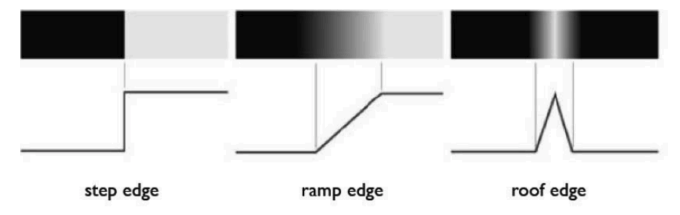
\includegraphics[width=0.75\linewidth]{images/pixel_intensity.png}
    \caption{Representation of the three types of edge that can be found in image analysis.\\Source: \cite{niebles2012edge}}
    \label{fig:pixel_intensity}
\end{figure}

\subsubsection{Gradient Computation}\label{sec:deriv_mask}

In HOG, a derivative mask (also known as a filter or kernel) is used to compute gradient information from an image \cite{dalal_2005_histograms} by performing convolution, the process of adding each element of the image to its local neighbors, weighted by the mask \cite{niebles2012edge}, as shown in equation \ref{eq:convolution}, where $I$ is the image matrix, $K$ the mask's matrix and $k$ - the "radius" of K (the distance from the center element to an edge element). 

\begin{equation}\label{eq:convolution}
    F(x,y) = \sum_{i=-k}^{k} \sum_{j=-k}^{k} I(x+i,y+j) \cdot K(i,j)
\end{equation}

%TODO: Make this discrete convolution equation actually make sense

The authors of HOG found that a simple 1D derivative mask of form $[-1,0,1]$, formally called a central discrete derivative \cite{niebles2012edge}, while being much less computationally expensive than 3x3 Sobel or 2x2 diagonal masks, also performed the best \cite{dalal_2005_histograms}.

Convolution on an image $I$ with the aforementioned 1D mask yields a new image $F_y$ defined in \ref{central_1} and convolution with the transposed, or, in other words, "flipped" over its main diagonal, 1D mask yields an image $F_x$ as defined in \ref{central_2}.

\begin{equation}\label{central_1}
    F_{y}(x_{m},y_{n}) = \frac{ \partial I(x_{m},y_{n}) }{ \partial x } \approx |\ I(x_{m}-1,y_{n})-I(x_{m}+1,y_{n})\ | 
\end{equation}
\begin{equation}\label{central_2}
    F_{x}(x_{m},y_{n}) = \frac{ \partial I(x_{m},y_{n}) }{ \partial x } \approx |\ I(x_{m},y_{n}+1)-I(x_{m},y_{n}-1)\ | 
\end{equation}

Notice however, that $x_m\pm 1$ and $y_n\pm 1$ fall outside $I[0,w-1]\times[0,h-1]$ when $x_m=w-1$ and $y_n=h-1$ respectively. This means that gradient information at image boundaries is lost when using central finite differences for convolution \cite{shidlovskiy_2020_reducing}. The information loss is evident in the \href{https://github.com/scikit-image/scikit-image/blob/main/skimage/feature/_hog.py}{\_hog\_channel\_gradient} where the convolution output at boundary pixels defaults to zero. The nullified boundary pixels may disproportionately impact SVM performance when using smaller detection windows or block sizes, as these zeroed values constitute a larger fraction of the resulting histogram. To address this limitation, this investigation proposes a novel approach that combines central, forward, and backward finite differences \cite{niebles2012edge}.

Figure \ref{fig:finite_differences} displays the kernels of each of the finite differences. Because both forward and backward differences are not anchored around the central pixel, they can be used to yield the convoluted intensity values of pixels at the top \ref{finite_top} and left \ref{finite_left}, and bottom \ref{finite_bottom} and right \ref{finite_right} edges, respectively.

\begin{figure}
    \centering
    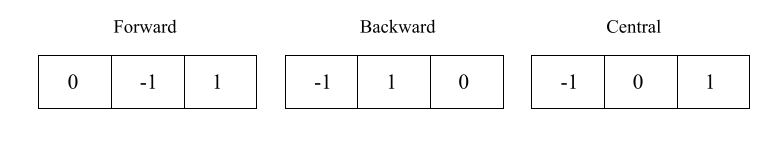
\includegraphics[width=0.75\linewidth]{images/finite_differences.png}
    \caption{Three types of finite differences and their corresponding derivative masks. Source: Image by me}
    \label{fig:finite_differences}
\end{figure}

\begin{equation}
    \label{finite_top}
    F_{x}[x_{m},0] =  | I(x_{m},1)-I(x_{m},0) | 
\end{equation}
\begin{equation}
    \label{finite_left}
    F_{y}[0,y_{n}] =  | I(1,y_{n})-I(0,y_{n}) 
\end{equation}
\begin{equation}
    \label{finite_bottom}
    F_{x}[x_{m},h] =  | I(x_{m},h)-I(x_{m},h-1) 
\end{equation}
\begin{equation}
    \label{finite_right}
    F_{y}[w,y_{n}] =  | I(w,y_{n})-I(w-1,y_{n}) 
\end{equation}

With the convoluted pixel values, or, in a sense, the changes in pixel intensity encoded into both $F_y$ and $F_x$ images, combining them into a single feature map $G$ of gradients, or vectors with an angle $\theta$, is as simple as applying the Pythagorean theorem \cite{shidlovskiy_2020_reducing}, as illustrated in figure \ref{fig:pythagorean}, where $ \text{magnitude} = | G(x_{m},y_{n}) | = \sqrt{ F_{y}(x_{m},y_{n})^2+F_{y}(x_{m},y_{n})^2 }$ and $\theta = \arctan \left( \frac{F_{y}(x_{m},y_{n})}{F_{x}(x_{m},y_{n})} \right) $

\begin{figure}
    \centering
    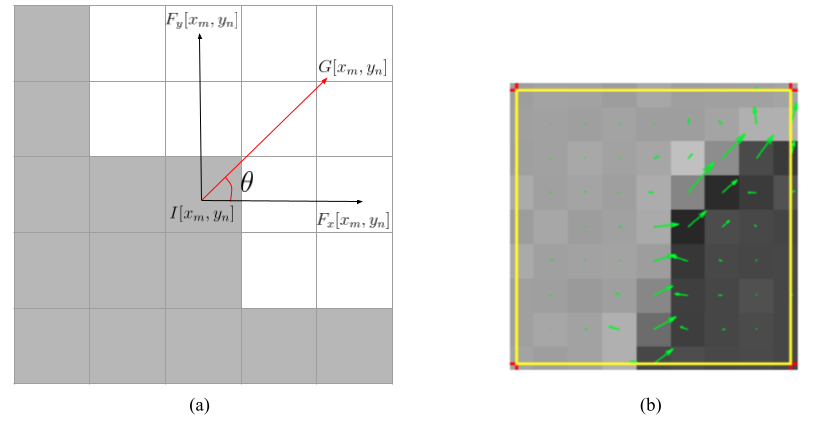
\includegraphics[width=0.75\linewidth]{images/pythagorean.png}
    \caption{(a) Calculation of gradient vector. Source: Image by me (b) Visualization of gradient vectors. Source: \cite{shidlovskiy_2020_reducing}}
    \label{fig:pythagorean}
\end{figure}

\subsubsection{Orientation Binning}

Orientation Binning hopes to achieve an encoding that is both sensitive to variations in local image content while remaining resistant to miniature changes in pose or appearance. This approach pools gradient orientation information locally, in a similar way that the SIFT feature detector does \cite{lowe_2004_distinctive}.

The process of orientation binning begins with dividing the constructed feature map of gradients into local spatial regions that the authors of the HOG algorithm called cells, as illustrated in figure \ref{fig:cells}.

\begin{figure}
    \centering
    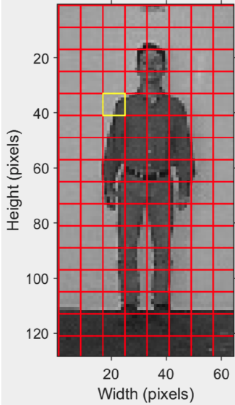
\includegraphics[width=0.3\linewidth]{images/cells.png}
    \caption{A 128x64 image divided into a grid of 8x8 pixel sized cells. Source: \cite{shidlovskiy_2020_reducing}}
    \label{fig:cells}
\end{figure}

Each pixel in a cell is characterized by its edge direction (0°-180°) and edge strength. The edge direction determines which oriented bin, $j$ (from equation \ref{eq:bin}), will receive the pixel's edge strength as its vote. These pixel-level measurements contribute to the cell's local feature vector of size $\omega$, which is essentially a histogram with $\omega$ bins evenly spaced across the 0°-180° range of possible edge orientations.

\begin{equation}
    \label{eq:bin}
    j = \left\lfloor  \left( \frac{\theta \omega}{180 \degree} \right) - \frac{1}{2}  \right\rfloor 
\end{equation}

\begin{figure}
    \centering
    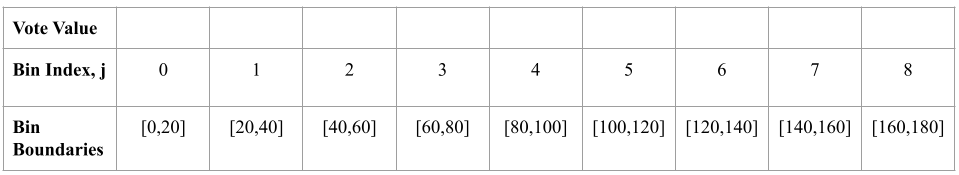
\includegraphics[width=0.75\linewidth]{images/histogram_bins.png}
    \caption{A histogram with 9 equally distributed bins. Source: Image by me}
    \label{fig:histogram_bins}
\end{figure}

While it is also viable to use 'signed' edge directions with a range of 0°-360°, it is generally unnecessary to distinguish between opposite edge directions since object classification is mainly based on detecting boundaries between regions of different intensities. Both edge directions of 90° and 270° convey the same boundary information, just with reversed intensity transitions \cite{shidlovskiy_2020_reducing}. The original HOG authors show that using signed edge directions not only fails to add useful information but actually decreases performance specifically in pedestrian detection \cite{dalal_2005_histograms}, presumably because the wide range of clothing and background color transitions obscure underlying shapes.

\subsubsection{Block Normalisation}
The magnitude of gradients can vary widely depending on local variations in illumination and foreground-background contrast. The authors of HOG thus found that local contrast normalization significantly contributes to classifier performance \cite{dalal_2005_histograms}, likely because it allows the classifier to focus on the structure of objects rather than brightness changes. It also ensures contrast invariance, balancing the influence of gradients in both high and low-contrast areas, preventing overemphasis on certain regions. Furthermore, normalization smooths the feature representation, reducing noise and making the extracted features more consistent across the image. By locally adapting to different image regions, normalization helps the classifier identify meaningful patterns and essential details.

Local contrast normalization addresses variations in illumination and contrast by first grouping the cell histograms into an unnormalized block descriptor vector, $\vec{f_{b}} = \{ b_{i} \ |\ i=1,2,\dots, c_w \cdot c_h \}$ (where $c_w$ and $c_h$ represent the number of cells in a block's width and height respectively), as illustrated in figure \ref{fig:normalisation}. While several normalization schemes exist ($\mathrm{L1}$, $\mathrm{L1-sqrt}$, $\mathrm{L2}$, and $\mathrm{L2-hys}$) \cite{dalal_2005_histograms} their impact on pedestrian detection performance is negligible. The original HOG authors found that all four schemes performed similarly, with $\mathrm{L2}$ and $\mathrm{L2-hys}$ showing only marginally better results \cite{dalal_2005_histograms}. This suggests that the choice of normalization scheme is less critical than other HOG parameters for pedestrian detection tasks.

\begin{figure}
    \centering
    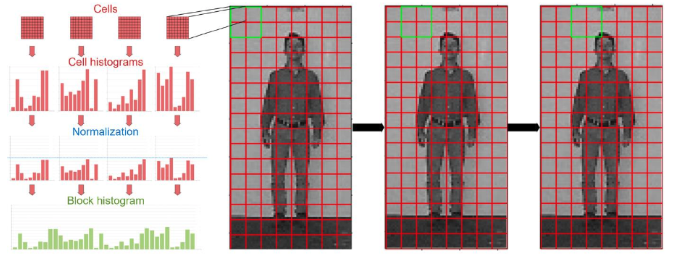
\includegraphics[width=0.75\linewidth]{images/normalisation.png}
    \caption{Construction of histogram blocks of size (2,2). Source: \cite{shidlovskiy_2020_reducing}}
    \label{fig:normalisation}
\end{figure}

One essential feature of grouping cell histograms into blocks is that the blocks themselves may overlap. Depending on the stride with which the block window moves, the horizontal and vertical overlaps will be $(1-\frac{\text{block width}}{\text{horizontal block stride}})\%$ and $(1-\frac{\text{block height}}{\text{vertical block stride}})\%$ respectively. While normalizing the same histograms in different block contexts may seem redundant, the authors of HOG found that the increased number of descriptor vectors $\vec{f_b}$ significantly improved performance \cite{dalal_2005_histograms}.

%TODO: Explain WHY it improved performance

\subsubsection{Feature Vector Dimensionality}\label{sec:feature_vector_dimensionality}

A sliding detection window is essential for object detection tasks like pedestrian classification because it allows the classifier to systematically examine all parts of the image at various positions and scales. Objects of interest, such as pedestrians, can appear at different locations, sizes, and orientations within an image, making it crucial to have a method that can effectively search across the entire image space. The sliding detection window of dimensions  $W_h$ and $W_w$ scans the image in a grid-like fashion, shifting over both horizontal and vertical axes. At each location, the window encompasses a region of interest containing a dense grid of overlapping blocks.

As the window moves across the image, the feature descriptors $\vec{f_b}$ within each block's region are computed, normalized, and combined into a larger feature vector, $\vec{L}$, as illustrated in figure \ref{fig:hog_pipeline}. The vector $\vec{L}$, representing the entire sliding window at that position, is used as input to the linear Support Vector Machine classifier to decide whether the window contains a pedestrian or not. 

\begin{figure}
    \centering
    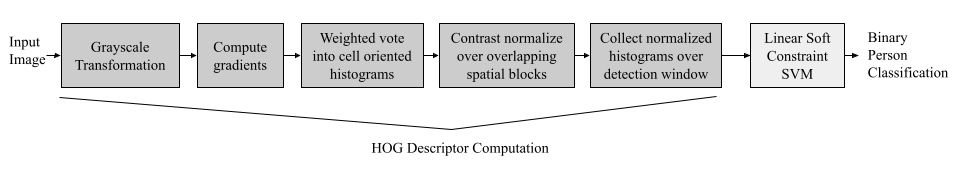
\includegraphics[width=1\linewidth]{images/HOG Pipeline.png}
    \caption{An overview of the HOG feature extraction chain. Source: Adapted by me from \cite{dalal_2005_histograms}}
    \label{fig:hog_pipeline}
\end{figure}

The dimensionality, $d$, of the vector $\vec{L}$ in essence describes the the total number of individual features, or gradients in a specific region of the image. Formally, it is said that the vector $\vec{L}$ belongs in a feature space of $d$ dimensions ($\vec{L} \in \mathcal{R}^{d}$). The higher the dimensions of this space, the more information a model has to distinguish between a pedestrian and the background or a humanoid silhouette (though this is not always the case, as explained in section \ref{sec:curse_of_dimensionality}). 

If we were to restrict the possible spatial block region's horizontal, $b_w$, and vertical, $b_h$, dimensions to even numbers, it could be easily expressed that the center coordinates, $x$ and $y$, of any block are bounded within $\left[ \frac{b_w}{2}; \frac{W_w}{c_w} - \frac{b_w}{2}\right]$ and $\left[ \frac{b_h}{2}; \frac{W_h}{c_h} - \frac{b_h}{2}\right]$ sets of cell values, respectively, as illustrated in figure \ref{fig:center_coords}

\begin{figure}
    \centering
    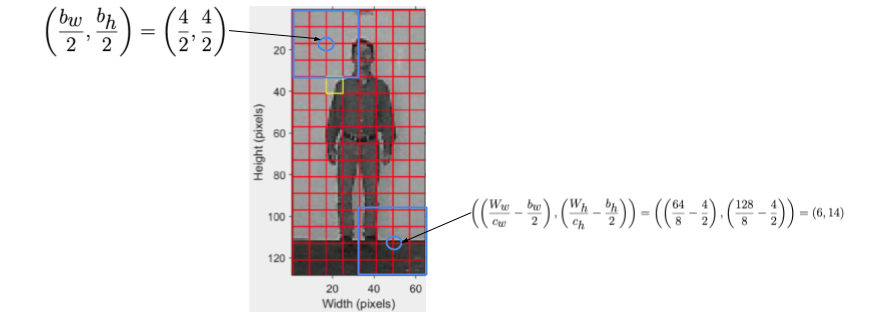
\includegraphics[width=1\linewidth]{images/Center Coordinates.png}
    \caption{A 128x64 sized image with cells that contain 8x8 pixels and blocks that contain 4x4 cells. The top left-most and bottom-right most block coordinates are each expressed using the aforementioned bounds. Source: Adapted by me from \cite{shidlovskiy_2020_reducing}}
    \label{fig:center_coords}
\end{figure}

The dimensionality $d$ of the final feature vector $\vec{L}$ depends on two factors: the size of each block descriptor $\vec{f_b}$ and the total number of blocks in the detection window. Each block descriptor's size is determined by the number of cells in the block ($c_w\cdot c_h$) multiplied by the number of orientation bins per cell ($\omega$). The number of blocks is determined by how many times a block can be shifted within the window using the horizontal and vertical stride values ($s_w$ and $s_h$). These relationships are formalized in equation \ref{vector_dimensions}.

\begin{equation}
    \label{vector_dimensions}
    \begin{split}
    d &= \left\lfloor \frac{\frac{W_w}{c_w}-2\cdot\frac{b_w}{2}+1}{s_w} \right\rfloor\left\lfloor \frac{\frac{W_h}{c_h}-2\cdot\frac{b_h}{2}+1}{s_h} \right\rfloor\cdot b_w b_h\omega \\ &= \left\lfloor  \frac{W_w- c_w(b_w-1)}{s_w c_w}  \right\rfloor \left\lfloor   \frac{W_h -c_h(b_h -1)}{s_h c_h} \right\rfloor b_w b_h\omega
    \end{split}
\end{equation}

\subsection{Supervised Machine Learning}\label{sec:supervised_ml}

Machine Learning (ML), on a surface level, is the study of algorithms that are designed to produce outputs without an explicit instruction set generated by a person but rather with reference to the patterns or correlations found in data \cite{what_is_ml}. 

In that respect, supervised ML algorithms are a subset of ML algorithms which attempt to make predictions from data \cite{supervised_learning}. Such algorithms rely on labeled training datasets, or data sets which provide the correct outputs that an algorithm should produce for each input data point \cite {supervised_learning}. 

Supervised ML applications include classifiers, such as a pedestrian detection program, which learn from previously annotated data in the hope of predicting the "class" to which future input data will belong. \cite{derek_2020_svm}. For example, a good pedestrian classifier should be able to predict whether an image's window belongs to the class of windows that contain a pedestrian or to the class of windows that do not contain a pedestrian.

Classifier training data is formally defined as $D={ (x_{1},y_{1}),\dots,(x_{n},y_{n}) }$, where each feature vector $x$ belongs to a $d$-dimensional space ($x\in \mathcal{R}^d$) and each label $y$ belongs to a label space $\mathcal{C}$ \cite{supervised_learning}. For pedestrian detection, which is a binary classification problem, the label space contains just two values: $+1$ for pedestrians and $-1$ for non-pedestrians \cite{cornell_svm}. Since each feature vector $x$ corresponds to a HOG descriptor $\vec{L}$, any change in the HOG parameters discussed in section \ref{sec:feature_vector_dimensionality} alters the dimensionality of $\vec{L}$ and consequently requires training a new classifier model with appropriately dimensioned feature vectors.

\subsection{Support Vector Machines}

Support Vector Machines (SVM) are widely adopted supervised machine learning algorithms, particularly well-suited for high-dimensional feature spaces like those generated by HOG descriptors \cite{ng_support}. While other classification algorithms exist, such as decision trees \cite{cornell_decision_trees}, naïve bayes \cite{cornell_naive_bayes}, and deep neural networks \cite{cornell_nn}, SVMs are especially effective at finding optimal separation boundaries in high-dimensional spaces \cite{chang_lin_2011_libsvm}. Their effectiveness has been demonstrated across various domains, from medical applications like brain disorder diagnosis \cite{derek_2020_svm} and neuroimaging analysis \cite{svm_mri} to computer vision tasks, where they have become the standard classifier for HOG-based pedestrian detection \cite{dalal_2005_histograms}.

An SVM finds the optimal boundary (hyperplane) to separate data points of different classes \cite{derek_2020_svm}. This hyperplane is mathematically defined as $\mathcal{H}={ x|w^\top x + b = 0 }$, where $w$ is the weight vector and $b$ is the bias \cite{cornell_svm_notes}. While other algorithms like the Perceptron \cite{cornell_perceptron} also find separating hyperplanes, SVMs are distinguished by their goal of maximizing the margin—the distance between the hyperplane and the nearest data points (called support vectors) from each class \cite{ng_support}. Figure \ref{fig:hyperplane} illustrates this concept in two dimensions, where the hyperplane becomes a line, $w$ represents the vector perpendicular to this line, and $b$ determines the line's intercept with the y-axis.

\begin{figure}
    \centering
    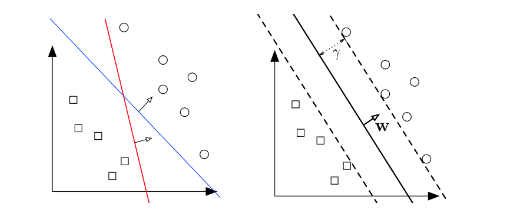
\includegraphics[width=0.75\linewidth]{images/hyperplane.png}
    \caption{A 2 dimensional space, where each data point has 2 features (one abscissa and one ordinate component) (Left:) Two different separating hyperplanes for the same data set (the multiple possibles hyperplanes of, for example, the perceptron algorithm). (Right:) The maximum margin hyperplane (the only possible hyperplane of the SVM algorithm). Source: \cite{cornell_svm_notes}}
    \label{fig:hyperplane}
\end{figure}

A hyperplane with the maximum possible margin between its support vectors is incredibly useful as it increases the likelihood of producing a generalized classifier, which can accurately separate unseen data points \cite{cornell_svm}. By expressing the distance between any point and that point's projection in the hyperplane, as illustrated in figure \ref{fig:hyperplane_geometry}, with the two variables that define the hyperplane itself (the weight and the bias), we get a definition of the margin, $\gamma$ in \ref{margin_expr} \cite{cornell_svm_notes}

\begin{equation}\label{margin_expr}
    \gamma(w,b)=\min_{x\in D} \frac{|w^\top x + b|}{||w||_{2}}
\end{equation}

\begin{figure}
    \centering
    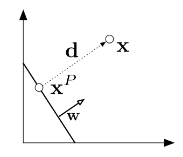
\includegraphics[width=0.35\linewidth]{images/hyperplane_geometry.png}
    \caption{The projection of a data point onto the hyperplane. Source: \cite{cornell_svm_notes}}
    \label{fig:hyperplane_geometry}
\end{figure}

With a defined margin, finding the optimal hyperplane can be formulated as a concrete optimization problem: maximize the margin $\gamma$ while ensuring all data points lie on the correct side of the hyperplane based on their class labels. The latter requirement is expressed mathematically as the inequality in equation \ref{hyper_inequality} \cite{ng_support}. For any data point $x_i$, the expression $w^\top x_i + b$ determines its position relative to the hyperplane $\mathcal{H}$: positive values indicate $x_i$ lies above $\mathcal{H}$, while negative values indicate it lies below. Therefore, when this expression is multiplied by the class label $y_i$ (which is either +1 or -1), the result should be positive for correctly classified points, providing a mathematical foundation for the optimization constraint.

\begin{equation}\label{hyper_inequality}
y_{i}(w^\top x_{i}+b)\ge 0 \quad 
\end{equation}
%TODO: Should I expand more on the concrete form of how this optimization problem looks?

\subsubsection{Soft SVM Constraints}\label{sec:soft_constraint_svm}
% Improve this paragraph
Traditionally obtaining the largest possible margin $\gamma$ would be a quadratic programming problem \cite{quadratic_programming} (as the goal of maximizing $\gamma$ is primarily anchored around minimizing $||w||_{2}$ from the equation in \ref{margin_expr} with the linear constraint in \ref{hyper_inequality}). While an SVM model's hyperplane such a "hard" constraint in \ref{hyper_inequality} could, in theory, be found found using either QCQP \cite{cornell_svm_notes} or SMO \cite{chang_lin_2011_libsvm} algorithms, in practice pedestrian datasets are incredibly noisy, as mentioned in section \ref{sec:introduction}, while also containing humanoid figures which closely approximate the features of a pedestrian \cite{inria_improved}, as visualized in figure \ref{fig:manequin_features}. Because of noise and obfuscation in real world pedestrian data, an SVM with a hard linear constraint would fail to compute the optimal hyperplane as there would be a significant number of outliers or data points which share features common to both classes, as illustrated in figure \ref{fig:outliers}. Instead, in the hope of finding a hyperplane that achieves the best realistically possible classification accuracy, an SVM with a soft constraint, which does allow for some degree of error while maximizing $\gamma$, ought to be used \cite{dalal_2005_histograms} \cite{cornell_svm_continued}.

\begin{figure}
    \centering
    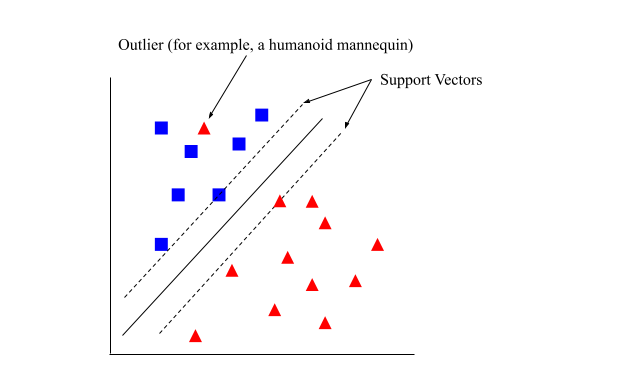
\includegraphics[width=0.75\linewidth]{images/outliers.png}
    \caption{A Data set with two classes and an outlier. Source: Image by me}
    \label{fig:outliers}
\end{figure}

\begin{figure}
    \centering
    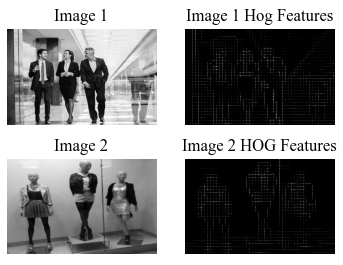
\includegraphics[width=0.75\linewidth]{images/features.png}
    \caption{(Image 1: ) An Image containing three people/pedestrians in a building. Source: \href{https://www.istockphoto.com/photo/business-people-taking-a-break-gm639259132-115111535}{istockphoto.com} (Image 2:) An Image containing three mannequins in a store window. Source: \href{https://theshopcompany.com/blog/Mannequins_and_Dressforms_Who_Uses_What}{theshopcompany.com} (Image 1 and 2 Hog Features): Computed HOG Features of Image 1 and Image 2. Source: Image by me}
    \label{fig:manequin_features}
\end{figure}

% TODO: Will I even be able to explain how to maximise the margin?

\subsection{The Curse of Dimensionality}\label{sec:curse_of_dimensionality}

While it would be reasonable to intuitively to assume that the more information, or vector dimensions, a machine is provided during training, the more accurate it would be at classification tasks, the classic "curse of dimensionality" problem shows that this is not necessarily the case \cite{jain_1982_39} \cite{friedman_1997_on}, as overfitting, the process of fitting to noise rather than underlying patterns, \cite{overfitting} occurs when the amount of "specific information" (the dimensions of each data point's vector $\vec{L}$) is significantly greater than "global information" (the amount of data points in a data set) \cite{overfitting} \cite{liu_2016_overfitting}, as shown in figure \ref{fig:curse_dim}. 

\begin{figure}
    \centering
    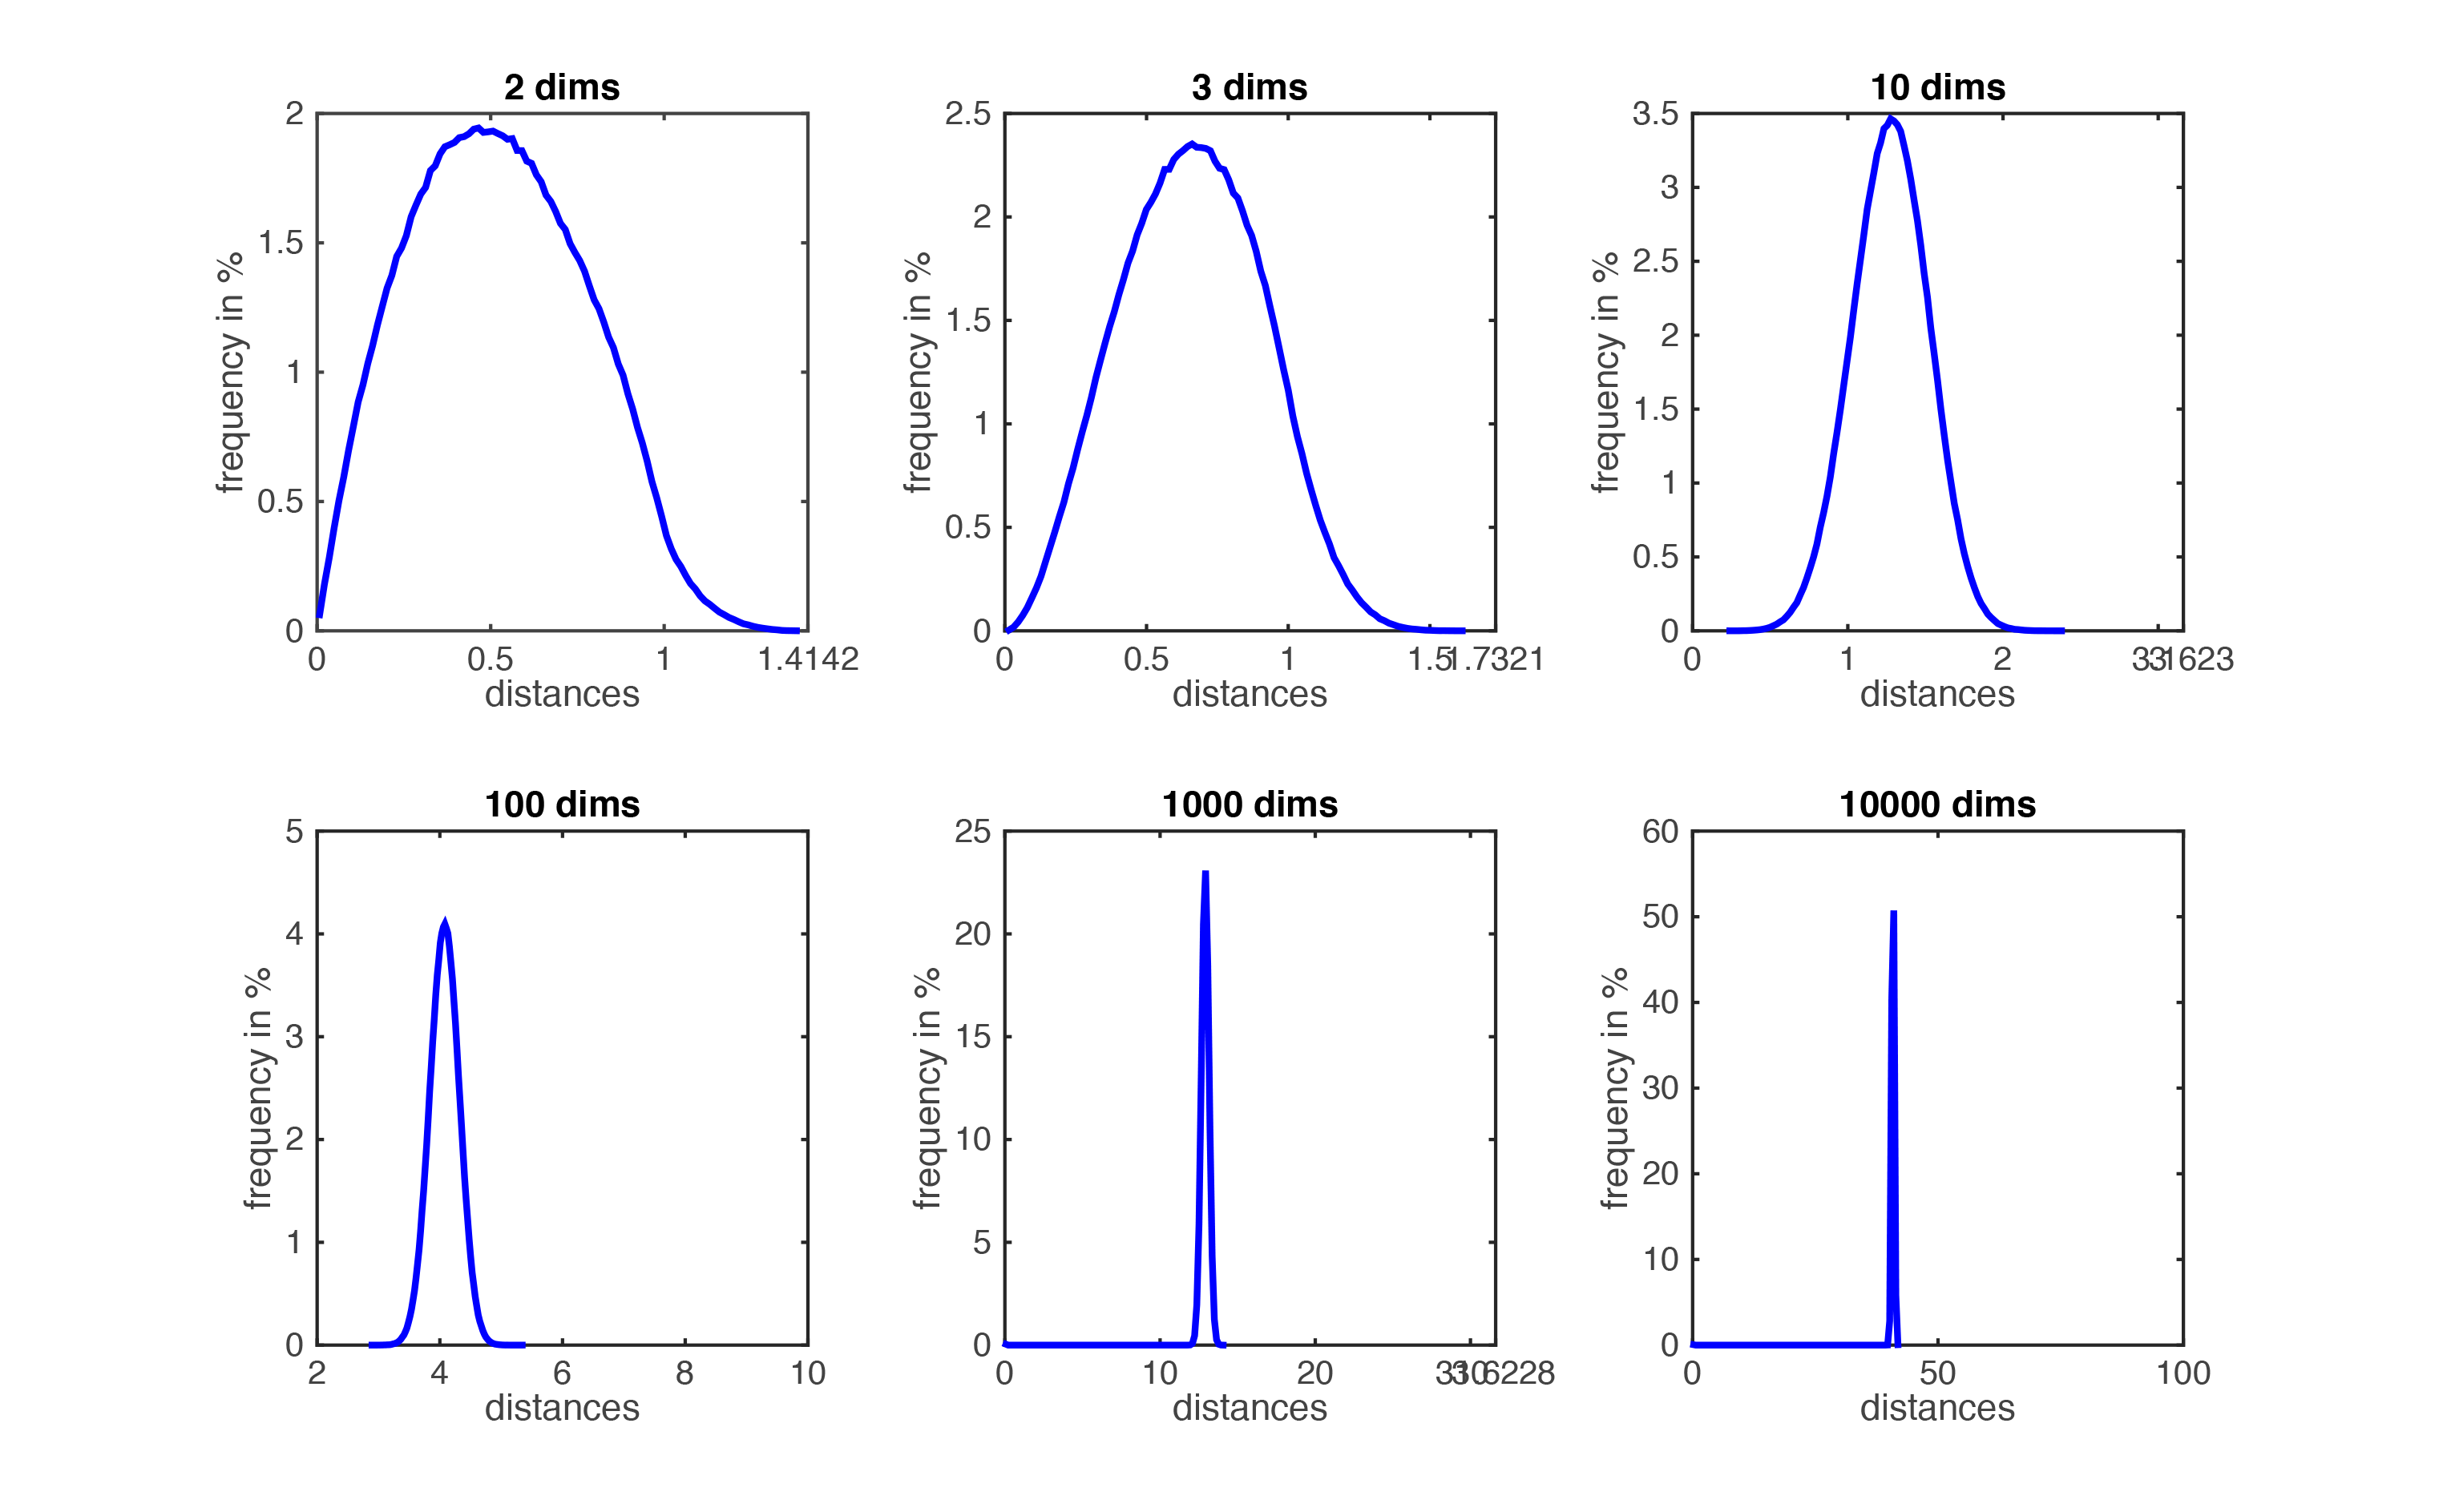
\includegraphics[width=\linewidth]{images/cursefigure.png}
    \caption{Multiple graphs which demonstrate the "curse of dimensionality". The histogram plots show the distributions of all pairwise distances between randomly distributed points within $d$-dimensional unit squares. As the number of dimensions $d$ grows, all distances concentrate within a very small range. Source: \cite{cornell_curse_notes}
}
    \label{fig:curse_dim}
\end{figure}


